\documentclass[a4paper]{scrartcl}

\usepackage[ngerman]{babel}
\usepackage[utf8]{inputenc}  % Umlaute etc. verwenden
\usepackage[final]{graphicx}    % Grafiken einbinden
\usepackage{url}


\usepackage[pdftex,
    pdftitle={Hier soll der Titel hin},
    pdfauthor={Niklas Weimann}]{hyperref}


\setcounter{secnumdepth}{3}


\begin{document}

% Der Titel der Seminararbeit, sowie der Autor
\title{Hier soll der Titel hin}
\author{Niklas Weimann}
\date{\today}

\maketitle


\tableofcontents
\newpage



\section{Einleitung}
"Pink + Purple == Fuchsia (a new Operating System)"\cite{GoogleLLC.} So beschreibt Google ein neues Betriebssystem, das sich zur Zeit noch in aktiver Entwicklung befindet. Das genaue Ziel dieses neuen Betriebssystems ist bis jetzt nur Google selbst bekannt, aber es gibt in den Medien einige Spekulationen darüber, wieso dieses System neu entwickelt wird und was die Absicht dahinter sein könnten. Dabei taucht immer wieder die Vermutung auf, dass Google Fuchsia als Ersatz für seine bereits existierende Betriebssysteme Android und ChromeOS entwickelt. Außerdem soll Fuchsia so modular sein, dass es sowohl auf IoT Hardware, als auch auf einem vollwertigen Desktop Computer zum Einsatz kommen kann. Google hat für die Entwicklung des neuen Systems einen Kernel basierend auf dem Littlekernel Projekt entwickelt. Littlekernel wird bereits für den Android bootloader und das Android Trusted Execution Enviroment eingesetzt. Unter Fuchsia bildet Zircon, das auf Littlekernel basiert, die Basis für das neue Betriebssystem. Im Gegensatz zu Linux setzt Fuchsia jedoch auf einen Mikrokernel, was bedeutet, dass der Kernel nur die wichtigsten Funktionalitäten implementiert und alles weitere in den Benutzerbereich ausgelagert wird, dies hat zur Folge, dass sich Fuchsia stark von Linux, das auf einen monolithischen Kernel setzt, unterscheidet.

Diese Seminararbeit beleuchtet die wesentlichen Konzepte, in denen sich Fuchsia und Android beziehungsweise ChromeOS unterscheiden. Dabei werden zunächst die wichtigsten Unterschiede zwischen dem Fuchsia Kernel und dem Linux Kernel beleuchten. Anschließend wird ein Überblick über das Komponenten Framework, dass eine wesentlich Rolle unter Fuchsia spielt, geben sowie eine Bewertung über die Vor und Nachteile dieses Frameworks. Zum Schluss wird die Treiberverwaltung der verschiedenen Systeme, sowie die verschiedenen Dateisysteme verglichen.
\section{Zircon}
Fuchsia setzt auf den Microkernel Zircon, der vor seiner Umbenennung Magenta hieß. Zircon entstand aus Little Kernel, einem Projekt von Travis Geiselbrecht. Der Kernel wurde so designet, dass er sowohl auf IoT Hardware, als auch auf Desktop Computern eingesetzt werden kann. \cite{DaveAltavilla.30.Juni2019} Die Systemaufrufe, die Zircon zur Verfügung stellt, sind bis auf wenige Ausnahmen alle asynchron und blocken somit nicht den aufrufenden Thread, dies ermöglicht eine effizientere Abarbeitung der Jobs.
\subsection{Kernel Objects und System Calls}
Alle System Calls an den Zircon Kernel sind, bis auf wenige Ausnahmen asynchron und unterbrechbar, somit ist es möglich, dass der Thread während der Ausführung auf eine andere CPU migriert werden kann, was eine erhebliche Verbesserung der Performance zur folge hat.
Handles werden von System Calls zurückgegeben, falls diese ein Kernel Objekt erstellt haben (z.b. zx\_event\_create() + zx\_process\_create() + zx\_thread\_create()). Im Usermode ist dieses Handle eine 32 Bit Zahl, wobei die letzten 2 LSB bei validen Handles immer gesetzt sind und die Zahl 0 ein ungültiges Handle repräsentiert. Ein Handle hat nur für den jeweiligen Prozess eine Bedeutung, der es angefordert hat, in einem anderen Prozess kann dieses Handle auf ein anderes Kernel Objekt zeigen oder ungültig sein. Ein Prozess kann mehrere Handles haben, um auf das selbe Kernel Objekt zuzugreifen, wobei sich hierbei dann meist die jeweiligen Zugriffsrechte unterscheiden. Die Zugriffsrechte, die ein Handle auf ein Kernel Objekt hat, werden im Kernel gespeichert. Der Kernel hat für jedes Handle ein C++ Objekt, das erstens eine Referenz auf das Kernel Objekt hat, zweitens eine Liste mit allen Rechten die das Handle hat und drittens eine Referenz auf den Prozess, zu dem es gehört. Diese Zugriffsrechte können einschränken werden, indem mittels zx\_handle\_duplicate() \cite{https://fuchsia.dev/fuchsia-src/reference/syscalls/handle_replace} oder mittels zx\_handle\_replace() \cite{https://fuchsia.dev/fuchsia-src/reference/syscalls/handle_replace} ein neues Handle erstellt wird, dass eine Untermenge der Rechte des Ursprünglichen Handles besitzt.
Jedes Kernel Objekt kann eine Reihe an Outputs haben, sogenannte Signale. Jedes Signal kann nur eine ein Bit Information repräsentieren, wobei pro Objekt bis zu 32 Signale möglich sind. Diese Signale können mittels System Calls erwartet werden. Diese Signale repräsentieren sozusagen den Zustand, in dem sich das Kernel Objekt befindet.
Unter Linux hingegen gibt es keine Kernel Objekte und keine Handles. Systemcalls unter Linux sind relativ primitiv umgesetzt, es wird bei einem Systemcall nicht überprüft, ob ein Aufrufer die entsprechenden Rechte hat. Wenn ein Systemcall aufgerufen wird, dann werden die entsprechenden Daten, sowie der passende OP-Code einfach in die entsprechenden Register kopiert. Diese Implementierung ist zwar wesentlich einfacher umzusetzen, als das Handle Konzept von Zircon.
% Evtl. weiter ausarbeiten 
\subsection{Scheduling}
Bei Zircon läuft auf jeder CPU ein unabhängiger Scheduler, jedoch können die Scheduler untereinander kommunizieren, um Überlasten zu erkennen und Prozesse bei Bedarf auf eine andere CPU migrieren zu können, wobei Prozesse auch selbst angeben können, auf welcher CPU sie ausgeführt werden sollen.

Jeder Scheduler hält dabei für jede der 32 möglichen Prioritäten eine Warteschlange vor, in der die Prozesse auf die Ausführung warten, solange sie nicht den Status \"Blocked\" haben. Ein geblockter Prozess wird in eine Warteschlange für die entsprechende Ressource gepackt und nimmt nicht weiter am Scheduling teil, bis er entblockt wird. Nachdem die Ressource frei ist und der Prozess entblockt wurde, wird der Prozess direkt an den Anfang der entsprechenden Warteschlange für seine Prioriät eingefügt, sodass er sein komplettes Zeitintervall ausnutzen kann. Hat er das Zeitintervall aufgebraucht, wird er wieder ans Ende der Warteschlange eingefügt.

Welche Priorität ein Prozess bekommt hängt dabei von drei Faktoren ab, erstens gibt es eine Base Priorität, die frei gewählt werden kann, zweitens gibt es einen Prioritäts Boost und drittens eine Prioritätsvererbung.
Der Prioriätatsboost wird auf die Basis Priorität addiert und wird um eine Prioritätsstufe erhöht, wenn der Prozess entblockt wird, nachdem er auf eine Ressource gewartet hat, wohingegen die Prioritätsstufe um eines verringert wird, wenn der Prozess vor Ende seines zugewiesenen Zeitintervalls ein Resheduling anfordert oder wenn er das komplette Zeitintervall ohne Unterbrechung gerechnet hat.

Die Prioritätsvererbung wird eingesetzt, um Prozesse, die auf eine Ressource warten, die jedoch durch den aktuellen Prozess blockiert ist, schneller an die Ressource kommen zu lassen, da der aktuelle Prozess die Priorität des wartenden Prozesses erbt, wird der aktuelle Prozess häufiger aufgerufen und kann somit schneller terminieren.

Die Prioritätsberechnung ist wichtig, da Zircon im Gegensatz zu Linux auf einen Fairen Scheduling Algorithmus setzt, um die limitierte CPU Zeit auf die Prozesse zu verteilen. Die Warteschlangen für die einzelnen Prioritätsstufen werden im Round Robin Verfahren durchlaufen, somit ist sichergestellt, dass alle Threads (nach ausreichend langer Wartezeit) einmal in ausgeführt werden und nicht durch immer neu ankommende Threads mit einer sehr hohen Priorität verhungern.

Linux setzt in den aktuelleren Versionen auf einen Completly Fair Scheduling Algorithmus ähnlich zu dem von Zircon. Android hingegen setzt auf eine leicht abgewandelte des Linux Schedulers, hier werden die Prozesse in Gruppen aufgeteilt, um sicher zu stellen, dass Prozesse die im Vordergrund laufen häufiger CPU Zeit bekommen, als Prozesse, die im Hintergrund laufen. Dies wird im wesentlichen durch zwei Faktoren gesteuert, zum einen der Nice-Wert und zum anderen Cgroups.

Der Nice-Wert gibt an, wie nett ein Prozess zu den anderen Prozessen ist. Mit anderen Worten, je höher der Nice-Wert ist, um so seltener wird dieser Prozess vom Scheduler ausgewählt. Der Nice-Wert setzt also sozusagen die Priorität eines Prozesses nach unten ähnlich zu dem weiter oben erwähnten Prioritätsboost.

Cgroups (Control groups) sind ein von Linux bereitgestelltes System, um Prozesse zu Gruppieren und basierend auf diesen Gruppen das Scheduling zu beeinflussen. Cgroups werden genutzt, um die Benutzeroberfläche von Android möglichst performant zu halten. Die Prozesse werden also entsprechend ihrer Aufgabe klassifiziert, somit kann eine Cgroup, die Beispielsweise aus Background Tasks besteht, so beschränkt werden, dass sie Maximal 5\% der CPU-Zeit erhalten, damit kann sichergestellt werden, dass immer ausreichend CPU-Zeit verfügbar ist, um die Benutzeroberfläche performant wirken zu lassen.
\section{Komponenten v2}
Komponenten spielen bei Fuchsia eine wichtige Rolle, da nahe zu alle Programme in Fuchsia als Komponente angesehen werden.
\subsection{Komponenten Einführung}
\label{sec:Components}
"Eine Komponente ist ein hermetisches zusammensetzbares isoliertes Programm" \cite{FuCHSIADOCS}, so wird der Begriff "Komponente" in der Fuchsia Dokumentation definiert. Komponenten können in jeder beliebigen Sprache implementiert werden, für die es einen Component-Runner gibt. Ein Component-Runner ist dabei für jede Programmiersprache nötig, die für die Implementierung einer Komponente verwendet wurden. Dieser hat Kenntnis darüber, wie eine Komponente ausgeführt werden kann, während der Komponenten-Manager weiß, was ausgeführt werden soll.

Jede Komponente läuft während ihrer Ausführungszeit in einer Sandbox, sie ist also komplett von anderen Komponenten isoliert, dies ermöglicht es, dass jede Komponente einen eigenen Lebenszyklus, Zustand und Funktionen hat, somit ist auch sichergestellt, dass diese Komponente keine ungewollten Auswirkungen auf andere Komponenten haben kann. Stürzt beispielsweise eine Instanz einer  Komponente ab, so kann sie einfach durch eine neue Instanz der selben Komponente ersetzt werden, dies erhöht signifikant die Stabilität des Systems.

Einzelne Komponenten werden durch ein Komponenten Manifest definiert, dieses enthält alle wichtigen Informationen, die der Komponenten-Manager oder der jeweilige Komponenten-Runner brauchen, um die Komponente erfolgreich ausführen zu können. \cite{https://fuchsia.googlesource.com/fuchsia/+/master/sdk/fidl/fuchsia.sys2/decls/component_decl.fidl} 
Die Eigenschaften im Komponenten Manifest umfassen unter anderem die Programm Eigenschaft,  die Informationen für den Komponenten-Runner bereitstellt, damit dieser die Komponente erfolgreich starten zu können. Außerdem wird im Komponenten Manifest festgelegt, welchen Speicher (mehr dazu in Kapitel \ref{sec:Dateisystem}),  welche Capabilities die Komponente benötigt, anbietet und weiterleitet (mehr dazu in Kapitel \ref{sec:Capabilities}), sowie wie einige weitere Eigenschaften, auf die hier nicht genauer eingegangen werden soll.

Um die Interoperabilität zwischen den Komponenten und verschiedenen Programmiersprachen zu ermöglichen, wurde für Fuchsia die Fuchsia Interface Definition Language Sprache entwickelt (mehr dazu in Kapitel \ref{sec:FIDL}).

\subsection{FIDL}
\label{sec:FIDL}
Die Fuchsia Interface Definition Language oder kurz FIDL entkoppelt die Definition von Inter Prozess Kommunikation (IPC) und der jeweiligen Implementierung der IPC Mechanismen. Dies kann an einem einfachen Echo Service leicht verdeutlicht werden. Mit FIDL ist es möglich, dass eine Komponente in C++ implementiert wird und mit einer Komponente kommuniziert die in Dart implementiert wurde. Zum Zeitpunkt der Erstellung dieser Seminararbeit werden C++, C, Rust, Go und Dart unterstützt. Für jede unterstütze Sprache muss ein ein entsprechender Übersetzer existieren, der die in der FIDL Datei definierten Strukturen in der entsprechenden Sprache erstellt. Die Fuchsia Dokumentation widmet diesem Thema einen ganzen Abschnitt, der für jede Sprache definiert, wie die Strukturen aus Fuchsia in die entsprechende Sprache übersetzt werden.\cite{https://fuchsia.dev/fuchsia-src/reference/fidl/bindings/overview}

Eine Komponente implementiert meist das ServiceProvider Interface, dieser Service ermöglicht es, dass die Interface Definition alle Service innerhalb der Komponente, basierend auf dem Servicenamen, ausgegeben werden können. Ein Service ist dabei die Implementierung eines Service Interfaces, das wiederum einzelne Protokolle definieren kann. Zum Beispiel definiert der Netstack Service die Protokolle name\_lookup und socket\_provider (Siehe Beispiel unter \cite{https://fuchsia.dev/fuchsia-src/concepts/components/services?hl=en}).

Eine Anwendung kann einen Service nutzen, indem sie über die von Zircon zur IPC zur Verfügung gestellten Channels eine Verbindung zu diesem Service herstellt. Über diese Verbindung kann können dann Nachrichten übermittelt werden. Dabei spielt das FIDL wire Format eine wichtige Rolle, dieses definiert, wie Objekte encodiert werden müssen, um sie so zu Versenden, dass der Service, der den Protokoll aufgerufen hat, die Nachricht wieder korrekt dekodieren kann.

Jeder Aufruf einer durch den FIDL Übersetzer definierten Methode ist asynchron, deshalb haben alle Methoden, die durch einen FIDL Übersetzer erstellt werden keinen Rückgabe Typen. Die Rückgabe an einen aufrufenden Prozess läuft mittels Callback ab, der, neben den definierten Parametern, auch als Parameter mit in die Methode gegeben wird. Dieser Callback kann ein oder mehrere Parameter haben, dieses entsprechen den Rückgabe Werten, die im FIDL Interface definiert wurden (Genauere Informationen: \cite{https://fuchsia.googlesource.com/docs/+/ea2fce2874556205204d3ef70c60e25074dc7ffd/development/languages/fidl/tutorial.md}).

Unter Android gibt es eine ähnliche Interface Sprache, um die Kommunikation zwischen Clients und Services zu definieren. Unter Android heißt diese Sprache Android Interface Definition Language kurz AIDL, sie definiert, ähnlich wie bei FIDL, ein Interface zur Inter Prozess Kommunikation. Im Gegensatz zu FIDL setzt AIDL jedoch eins zu eins auf die Java Syntax für seine Interfaces, während Fuchsia eine C++ ähnliche Syntax verwendet und dabei mehr Strukturen unterstützt, als AIDL. Somit ist in AIDL im Gegensatz zu FIDL die Anzahl der Rückgabewerte auf eins begrenzt.
\subsection{Komponenten Manager}
Der Komponenten Manager stellt in Fuchsia eine zentrale Rolle da, dieser verwaltet das Zusammenspiel zwischen den Komponenten(\ref{sec:Components}). Der Komponenten Manager ist einer der ersten Prozesse, die beim Booten des Systems gestartet werden, dies ist erforderlich, da der Komponenten Manager alle Komponenten startet, die in Fuchsia verwendet werden.

Der Komponenten Manager ist neben der Verwaltung von einzelnen Komponenten auch der Mittler zwischen Komponenten, er stellt zum Beispiel die Verbindung zwischen zwei Komponenten her. Wenn eine Komponente den Service einer anderen Komponente nutzen möchte, sendet die erste Komponente eine Anfrage nach der Ziel Komponente basierend auf der URL der Komponente an den Komponenten Manager, dieser wiederum kennt die zugehörige Komponente zu dieser URL und stellt die Verbindung entsprechend her. Beim Verbindungsaufbau kann es vorkommen, dass eine Komponente bereits gestoppt und somit persistiert wurde, wenn dies der Fall ist, sorgt der Komponenten Manager dafür, dass die Komponente wieder gestartet und der Zustand wieder hergestellt wird. Als Mittler validiert der Komponenten Manager jeden Aufruf zu einem Service basierend auf den Rechten, die im Komponenten Manifest festgelegt wurden.

Aufgrund seiner zentralen Rolle in Fuchsia hat der Komponenten Manager eine privilegierte Rolle, da er viele Sicherheits- und Stabilitätsrelevante Entscheidungen treffen muss. Unterstützt wird der Komponenten Manager dabei durch die bereits oben erwähnten Runner, welche das Wissen über die Ausführung einer Komponente kapseln.

Neben diesen Aufgaben kümmert sich der Komponenten Manager auch drum, dass die Komponenten in einer validen Topologie organisiert sind. Dazu verwaltet der Manager eine Baumstruktur für die Abhängigkeit der Komponenten, die in einer Eltern-Kind-Beziehung zueinander stehen können. Außerdem wird ein Routing Graph für die Capabilities der Komponenten verwaltet, dieser stellt da, wie einzelne Instanzen von Komponenten Zugriff auf die Dienste von anderen Komponenten erhalten, dabei ist jedoch zu beachten, dass immer nur Eltern Komponenten Zugriff auf die Dienste ihrer Kinder bekommen und nicht umgekehrt.

Der Komponenten Manager kümmert sich außerdem um den Lebenszyklus von Komponenten. Dabei ist wichtig zu wissen, dass eine Komponenten Instanz sich in einem von vier verschiedenen Zuständen befinden kann (Create, Start, Stop, Destroy).

Von einer Komponente kann eine neue Instanz erstellt werden, diese befindet sich initial im Zustand Create. In diesem Zustand wird der Instanz dann eine eindeutige ID zugewiesen, damit die Instanz immer wieder identifiziert werden kann. Anschließend wird die Instanz an die entsprechende Stelle im Komponentenbaum eingepflegt, somit kann auch der Routing Graph für die Capabilities angepasst werden. Im Zustand Start befindet sich die Instanz so lange, wie sie benötigt und ausgeführt wird, danach wechselt sie in den Zustand Stop, wenn die Instanz in den Zustand Stop wechselt, wird der aktuelle Zustand der Instanz persistiert, damit für die Komponente die Illusion ermöglicht wird, dass sie dauerhaft ausgeführt wird. Dies ermöglicht es auch, dass Komponenten beim wechseln auf ein anderes Gerät an der selben stelle fortgesetzt werden kann. Eine Komponente wechselt in den Zustand Destroy, wenn sie endgültig gelöscht wird, dabei werden alle Daten, die die Instanz betreffen, also auch der persistente Zustand gelöscht, damit existiert die Instanz der Komponente nicht mehr und es muss eine neue Komponenten Instanz erstellt werden.

\subsection{Capabilities}
\label{sec:Capabilities}
Capabilities, die eine Komponente zur Verfügung stellt können von anderen Komponenten benutzt werden, allerdings ist der Zugriff auf die Capabilities durch die im Komponentenmanifest festgelegten Rechte limitiert, die über den Komponentenmanager überwacht werden. Dazu gibt es im Komponentenmanifest verschiedene Keywords. Es gibt vier verschiedene Arten, die im Komponentenmanifest festgelegt werden können. Zu diesen Capabilities gehören Service, Protocol, Directory und Storage, wobei Service und Protocol, sowie Directory und Storage sehr ähnlich sind und sich nur marginal unterscheiden.


Service Capabilities erlauben es der Komponente A auf den FIDL Service von Komponente B zu zugreifen, während Protocol Capabilities nur den Zugriff auf ein einzelnes FIDL Protokoll erlauben. Der Unterschied wurde bereits in Kapitel \ref{sec:FIDL} erklärt.

Directory Capabilites erlauben es einer Komponente A auf einen Ordner der Komponente B zu zugreifen, wobei im Komponentenmanifest für jeden Ordner der Komponente festgelegt werden kann, dass sie diesen freigibt und ob sie diesen Ordner nur lesend oder auch schreibend zugreift. Storage Capabilities bieten für die Komponente, die auf den Storage zugreifen, einen isolierten Speicher, dazu benötigt sie eine Referenz auf eine Directory Capability, damit der Komponentenmanager für jede zugreifend Komponente einen neuen Ordner innerhalb des freigegebenen Ordners erstellen kann. Die Komponente, die den Ordner freigibt, kann dann auf die Daten jeder Komponente zugreifen, die den Storage genutzt hat, um Daten zu speichern, während die Komponente, die gespeichert hat, nur auf die Daten zugreifen kann, die sie selbst gespeichert hat. Dies ist der Unterschied zwischen Directory Capabilities und Storage Capabilities.
\begin{figure}
	\centering
	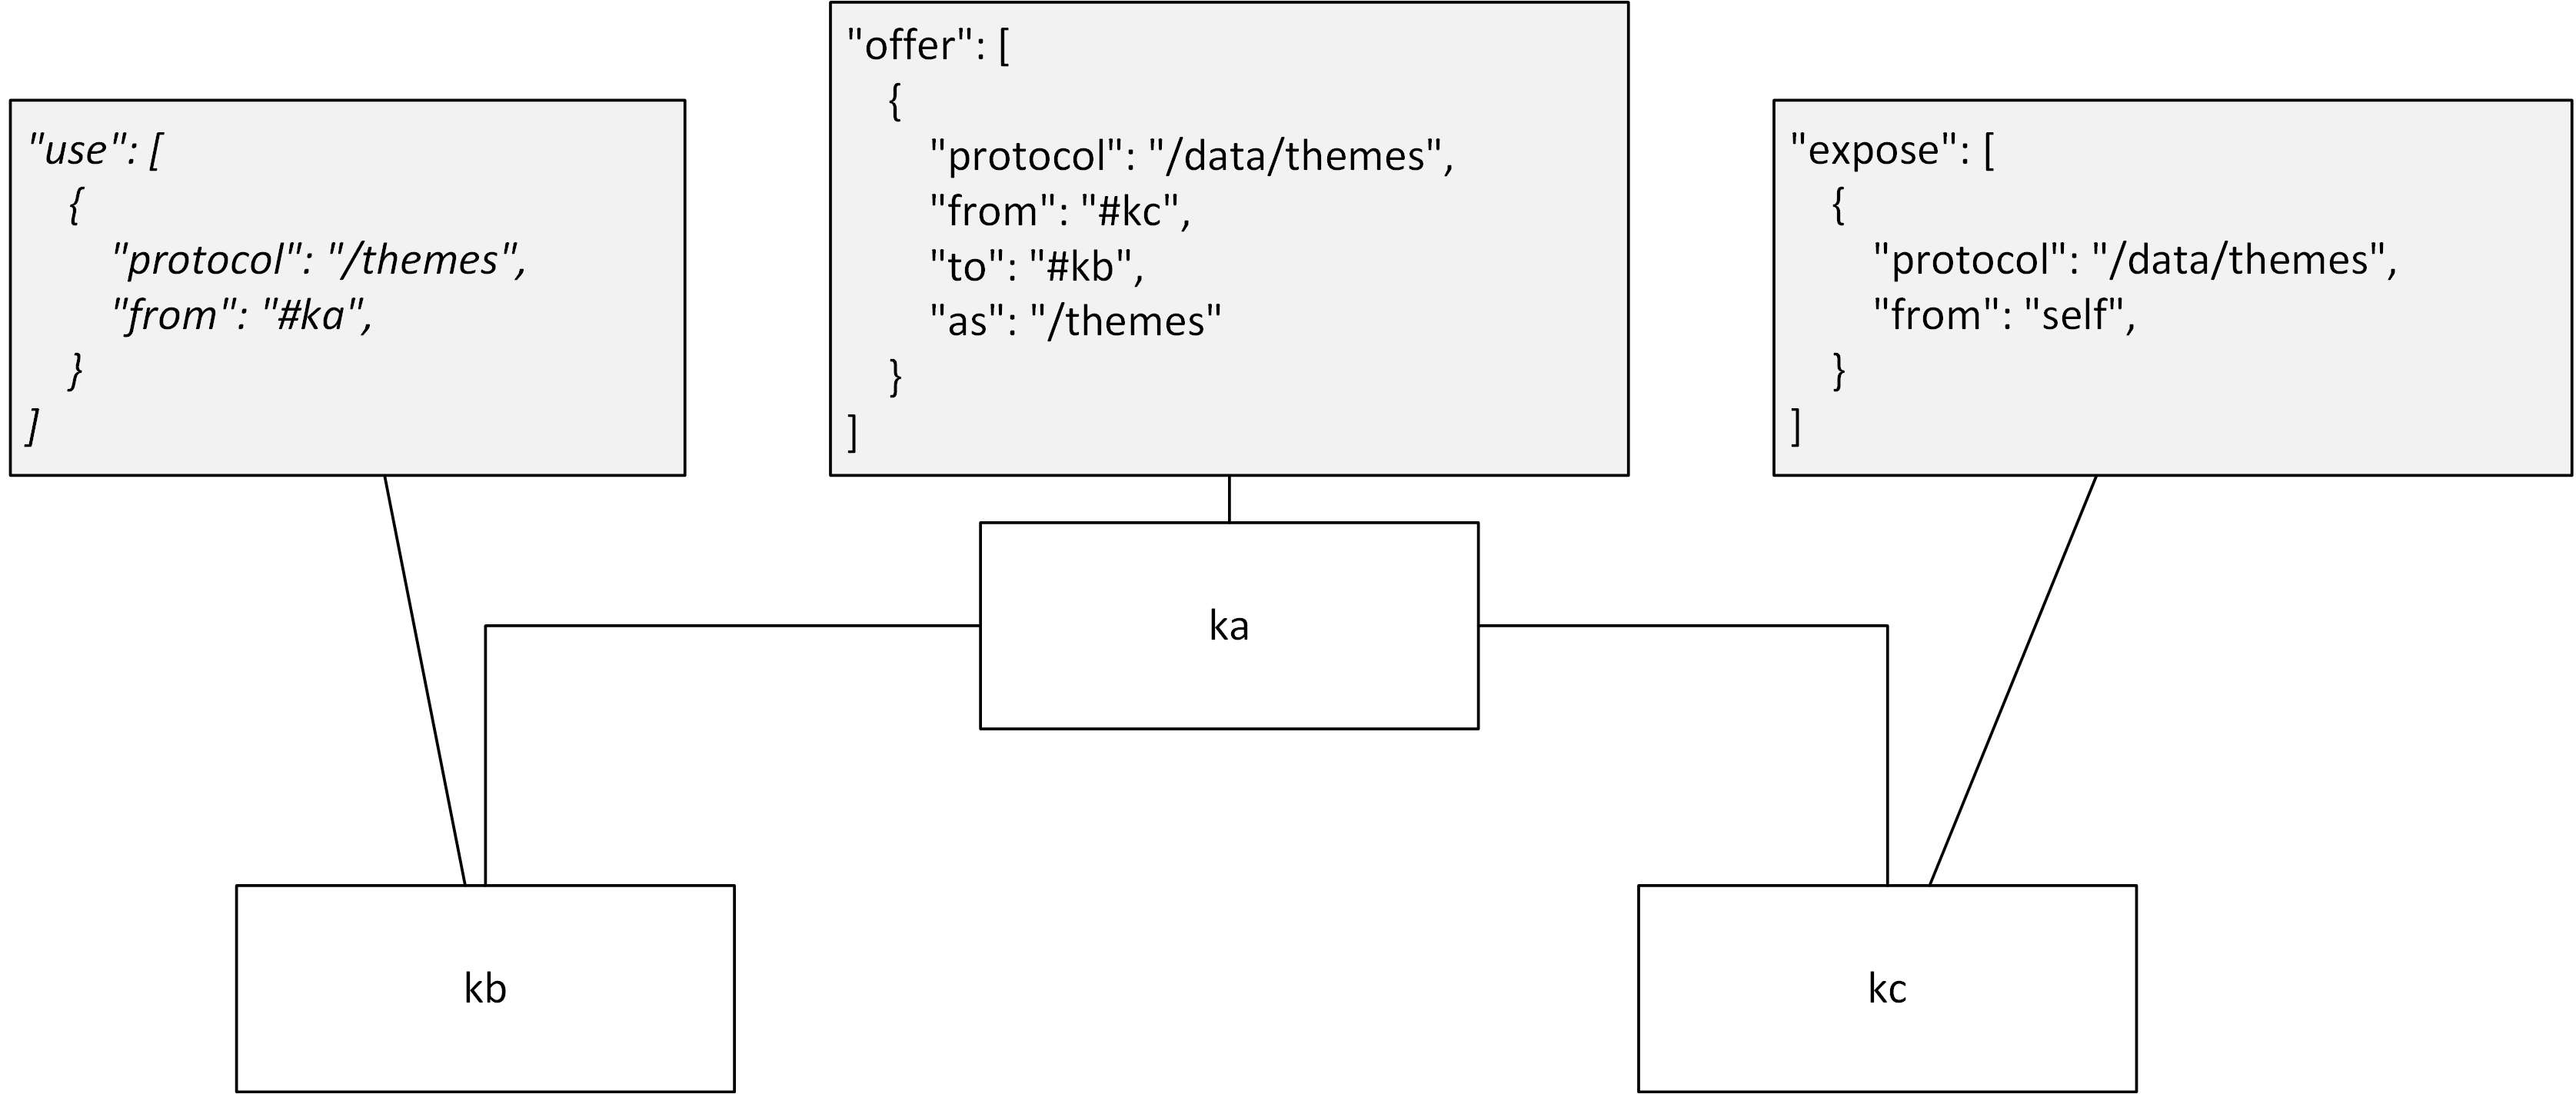
\includegraphics[width=1\textwidth]{figure/Capability_Routing}
	\caption[Kurzform vom Bild]{Graphische Darstellung des Capability Routing der Komponenten ka, kb und kc mit einem Ausschnitt aus den jeweiligen Komponentenmanifesten.}
	\label{abb:capabilityRouting}
\end{figure}
Capabilities können zugänglich gemacht, weitergeleitet und benutzt werden. Welche Komponente was mit welcher Capability macht, wird im Komponentenmanifest der Komponente angegeben. Wenn eine Komponente die Capabilities einer anderen Komponente nutzen möchte, kann sie dies mittels des use Schlüsselwortes im Komponentenmanifests angeben. Hier muss die Komponente den Typ der Capability sowie den Pfad zur Capability angeben, unter dem die Capability freigegeben wurde. Optional kann der Pfad im Komponentenmanifest mittels dem Schlüsselwort as auf einen anderen Pfad geleitet werden. Komponenten können mittels dem Schlüsselwort expose eine Capability an ihre Eltern weiter leiten und mittels offer an ihre Kinder Komponenten. Das Routing der Capabilites wird in Abbildung \ref{abb:capabilityRouting} genauer veranschaulicht. In diesem Beispiel gibt die Komponente kc ein FIDL-Protokoll unter dem Pfad /data/themes frei, während die Komponente ka dieses Protokoll an kb weiterleitet, indem sie es mittels offer ihrer Kind Komponente zur Verfügung stellt, dabei ändert sie den Pfad mittels as auf /themes. 

\subsection{Vergleich zu Komponenten}
Welche Vorteile bietet es, dass alles eine Komponente ist im Gegensatz zu Linux (Android)?
\section{Treiber}
\subsection{Verwaltung und Zugriff}
Treiber in Fuchsia beziehungsweise Zircon werden hierarchisch organisiert und möglichst kleinteilig pro Gerät gesplittet, somit wird eine unnötige Duplizierung von Programmcode verhindert.

Das Treiber-Framework in Fuchsia enthält unter anderem einen Gerätekoordinator, dieser  verwaltet eine Baumstruktur, die den Aufbau der Abhängigkeiten zwischen den einzelnen Treibern darstellt. So kann beispielsweise ein USB-Treiber als Elternknoten an einem PCI-Gerät hängen und selbst wieder einen Soundkarten Treiber als Kind haben, da an diesem PCI-Slot eine USB-Soundkarte hängt. Der Gerätemanager durchsucht /boot/driver und /system/driver nach Treibern, jeder dieser Treiber ist als Dynamic Shared Object (DSO) Implementierung. Damit der Geräte Koordinator bestimmen kann, welcher Treiber für welches Gerät verwendet werden kann, muss jeder Treiber eine Binding-Routine implementieren, die bestimmt, für welche Geräte dieser Treiber eingesetzt werden kann. Meist wird dazu die Vendor ID (VID) und Device ID (DID) verwendet, da diese in Kombination einzigartig für ein Gerät sind. 

Der Treiberbaum hat initial einen Root-PCI-Driver als Wurzel, dieser geht davon aus, dass sich in dem System ein PCI fähiges Gerät befindet, wenn es gefunden wird, dann wird es an diesen Treiber gebunden. Für alle Geräte, die wiederum physisch mit dem PCI Gerät verbunden sind, schaut der Gerätekoordinator in definierten Verzeichnissen nach, ob dort ein Treiber gefunden werden kann, dessen Binding Funktion für diese VID und DID ein positivies Ergebnis liefert. Jeder Pfad von der Wurzel des Baumes bis zu jedem Blatt wird vom Gerätekoordinator als Gerät betrachtet.

Basierend auf einer Systemrichtlinie splittet der Gerätekoordinator den Baum in einzelne Teilbäume, die jeweils innerhalb eines Geräte-Host-Prozesses (devhost) ausgeführt werden, durch die Teilung der Gerätetreiber in einzelne Gruppen soll eine höhere Stabilität und Sicherheit erzielt werden können.

Treiber können Metakommunikation für das Gerät bzw. den Treiber mittels eines FIDL-Protokols definieren. Das Lesen bzw. Schreiben von Daten an ein Gerät ist wie ein Lesezugriff bzw. Schreibzugriff auf eine Datei realisiert. Das Gerät ist dabei unter /dev/gemounted.
\subsection{Vergleich Treiber}
Der Linux Kernel besitzt kein System, dass Treiber in einzelne Prozesse trennt. Der monolithische Kernel von Linux lässt alle Treiber innerhalb des selben Prozesses laufen, dies hat zur Folge, dass ein Fehler in einem Treiber zu einem System Absturz führen oder eine Sicherheitslücke zu root Zugriff führen kann. Linux unterteilt Treiber in drei Kategorien: byteorientierte Geräte (z.B. Tastaturen), blockorientierte Geräte (z.B. Festplatten) und paketorientierte Geräte. Byteorientierte Geräte können nur jeweils ein Zeichen auf einmal ausgeben oder einlesen und sind als Dateien in das Dateisystem von Linux eingebunden. Während blockorientierte Geräte nur vielfache der spezifizierten Blockmenge lesen bzw. schreiben können, sind sie sowohl über einen Pfad im Dateisystem von Linux erreichbar, als auch über eine spezifische Datei im Dateisystem. 

Byteorientierte und blockorientierte Treiber werden unter Linux im chrdev bzw. blkdev Vektor gespeichert, sobald ein Gerät erkannt wird, wird der entsprechende Treiber in den Vektor eingefügt und ab dann werden die Major und Minor Nummer zur Identifizierung des Gerätes verwendet, wobei die Major Nummer den Type des Gerätes angibt (z.B. tty) und die Minor Nummer die einzelne Instanz des Gerätes identifiziert. Der Zugriff auf die Geräte erfolgt dann über eine Datei im Pfad /dev und mittels den regulären Systemcalls für Dateien können Daten von dem Gerät gelesen und an das Gerät gesendet werden.

Das Treibermanagement in Fuchsia und Linux unterscheidet sich also in zwei Aspekten. Fuchsia unterhält einen Baum, indem alle Geräte als Blätter repräsentiert werden, wohingegen Linux die Geräte in drei Klassen unterteilt und für jede Klasse einen eigenen Vektor mit den jeweiligen Geräten in dieser Klasse pflegt.

Außerdem sind Treiber unter Fuchsia im Userspace in einzelne Prozesse gekapselt, während Linux alle Treiber im Kernelspace ausführt. Der Userspace Ansatz hat zum Vorteil, dass die Auswirkungen von Bugs im Treiber oder aber auch absichtlich Manipulierte Treiber nur innerhalb ihres Prozesses Schaden anrichten können und keine Auswirkungen auf den Kernel an sich haben, wie es etwa bei Linux der Fall ist. Beim Linux Ansatz hingegen ist die Performance potentiell besser, da kein Kontextwechsel zwischen Kernelspace und Userspace notwendig ist, deshalb startet Fuchsia nicht für jedes Gerät einen neuen Prozess sondern kapselt mehrere Geräte in einen Prozess.

\section{Dateisystem}
\label{sec:Dateisystem}
\subsection{Dateisystem Architektur und Dateisystem}
Zircon hat kein eigenes Datei, sondern setzt darauf, dass ein Dateisystem im Benutzerbereich als Prozess zur Verfügung gestellt wird. Dadurch wird es theoretisch möglich, dass das Dateisystem während des laufenden Betriebes ausgetauscht und geupdatet werden kann. Diese Architektur setzt jedoch voraus, dass die Interaktion mit dem Dateisystem auf ein Interface beschränkt ist, dieses wird in Fuchsia mittels FIDL \cite{vglFIDLio} realisiert. Das Kommunikationsmodell für die Interaktion mit dem Dateisystem findet, da es sich immer um eine Kommunikation zwischen zwei Benutzerprozessen handelt, über Channels statt, wodurch ein Server/Client System entsteht. Der Prozess, der das Dateisystem zur Verfügung stellt, entspricht dabei einem Server und die Prozesse, die über die Channels, auf diesen Serverprozess zugreifen, um das Dateisystem zu nutzen, entsprechen in diesem Modell den Clients.

Dateisysteme haben typischerweise 2 Handels, eines, um mit dem Dateisystem selbst zu kommunizieren, und ein optionales, um mit dem Gerät zu kommunizieren, auf dem das Dateisystem gespeichert wird.

Wie sind Dateisysteme und das Dateimanagement realisiert?
\subsection{Cloudunterstützung}
Ledger ist ein auf Schlüsselwertpaaren basierender verteilter Speicher. Der Ledger erlaubt es basierend auf diesen Schlüsselwertpaaren Daten über einen Cloudspeicher mit anderen Geräten zu synchronisieren. Ein Eintrag besteht aus einem 16 Byte Schlüssel und einem beliebig großen byte Wert, der zum Zeitpunkt dieser Arbeit nur durch die Nachrichtengröße für FIDL Nachrichten limitiert ist.

Der Ledger selbst besteht aus drei Ebenen. Auf der ersten Ebene befindet sich der Lokale Client, dieser stellt eine FIDL Api für Komponenten zur Verfügung über die Änderungen, Löschungen und Abfragen von einzelnen oder mehreren Einträgen möglich sind. Wenn es durch die Ändernungen, die eine Komponente über die API angefragt hat zu einem Konflikt kommt, versucht der Client diesen Konflikt zu lösen, indem er die Strategie verwendet, die vorher von der Komponente angegeben wurde, wenn diese nicht möglich ist, wird die Anfrage zurück an die Komponente geleitet. Wenn die Anfrage nicht zu einem Konflikt führt, werden die Änderungen auf die zweite Ebene weitergegben. Auf der zweiten Ebene werden die Daten im Storage mittels eines atomaren Commits persistiert. Der Commit-Verlauf jeder Seite kann, ähnlich wie bei GIT, als DAG dargestellt werden. Der Storage speichert für jeden Commit zusätzlich die Meta Daten für die Einträge und sortiert sie in einen B-Baum ein. Wenn der Commit persistiert wurde, benachrichtigt der Storage die dritte und letzte Ebene, den Cloud Sync, dieser lädt den neuen Commit in die Cloud und sellt die Daten damit für die anderen Geräte zur Verfügung. Außerdem achtet der Cloud Sync auf Änderungen im Cloud Speicher und lädt die neuen Einträge herunter und pflegt sie in den Speicher ein, damit die Lokale kopie und der Cloud Speicher möglichst immer die selben Daten enthalten. 

Der Ledger unterstützt zwei verschiedene Betriebsmodi zum einen den Guest Mode und zum anderne den Regular mode. Im Guest mode hat der Ledger keine aktive Verbindung zur Cloud und speichert die Daten lediglich lokal. Im Regular Mode hat der Ledger eine aktive Verbindung zur Cloud und synchronisiert alle Geräte, die mit dem selben Benutzerkonto verbunden sind.
\subsection{Vergleich Filesystems}
Wie unterscheidet sich das Dateisystem von Linux (Andorid)?
\section{Zusammenfassung}
Grobe Zusammenfassung über die Unterschiede zu Linux (Android)

%***** Bibliographie  *****
%Die Literatur wird in einem eigenen Dokument im BibTeX Format erfasst: in diesem Fall: referenzen.bib
\bibliography{referenzen}
% --- Literaturstellen nummerieren
\bibliographystyle{plain}


\end{document}
